\chapter{The Third Attack}

Now that this treasure, which had so long been the object of the abbé’s
meditations, could insure the future happiness of him whom Faria really
loved as a son, it had doubled its value in his eyes, and every day he
expatiated on the amount, explaining to Dantès all the good which, with
thirteen or fourteen millions of francs, a man could do in these days
to his friends; and then Dantès’ countenance became gloomy, for the
oath of vengeance he had taken recurred to his memory, and he reflected
how much ill, in these times, a man with thirteen or fourteen millions
could do to his enemies.

The abbé did not know the Island of Monte Cristo; but Dantès knew it,
and had often passed it, situated twenty-five miles from Pianosa,
between Corsica and the Island of Elba, and had once touched there.
This island was, always had been, and still is, completely deserted. It
is a rock of almost conical form, which looks as though it had been
thrust up by volcanic force from the depth to the surface of the ocean.
Dantès drew a plan of the island for Faria, and Faria gave Dantès
advice as to the means he should employ to recover the treasure. But
Dantès was far from being as enthusiastic and confident as the old man.
It was past a question now that Faria was not a lunatic, and the way in
which he had achieved the discovery, which had given rise to the
suspicion of his madness, increased Edmond’s admiration of him; but at
the same time Dantès could not believe that the deposit, supposing it
had ever existed, still existed; and though he considered the treasure
as by no means chimerical, he yet believed it was no longer there.

However, as if fate resolved on depriving the prisoners of their last
chance, and making them understand that they were condemned to
perpetual imprisonment, a new misfortune befell them; the gallery on
the sea side, which had long been in ruins, was rebuilt. They had
repaired it completely, and stopped up with vast masses of stone the
hole Dantès had partly filled in. But for this precaution, which, it
will be remembered, the abbé had made to Edmond, the misfortune would
have been still greater, for their attempt to escape would have been
detected, and they would undoubtedly have been separated. Thus a new, a
stronger, and more inexorable barrier was interposed to cut off the
realization of their hopes.

“You see,” said the young man, with an air of sorrowful resignation, to
Faria, “that God deems it right to take from me any claim to merit for
what you call my devotion to you. I have promised to remain forever
with you, and now I could not break my promise if I would. The treasure
will be no more mine than yours, and neither of us will quit this
prison. But my real treasure is not that, my dear friend, which awaits
me beneath the sombre rocks of Monte Cristo, it is your presence, our
living together five or six hours a day, in spite of our jailers; it is
the rays of intelligence you have elicited from my brain, the languages
you have implanted in my memory, and which have taken root there with
all their philological ramifications. These different sciences that you
have made so easy to me by the depth of the knowledge you possess of
them, and the clearness of the principles to which you have reduced
them—this is my treasure, my beloved friend, and with this you have
made me rich and happy. Believe me, and take comfort, this is better
for me than tons of gold and cases of diamonds, even were they not as
problematical as the clouds we see in the morning floating over the
sea, which we take for \textit{terra firma}, and which evaporate and vanish as
we draw near to them. To have you as long as possible near me, to hear
your eloquent speech,—which embellishes my mind, strengthens my soul,
and makes my whole frame capable of great and terrible things, if I
should ever be free,—so fills my whole existence, that the despair to
which I was just on the point of yielding when I knew you, has no
longer any hold over me; and this—this is my fortune—not chimerical,
but actual. I owe you my real good, my present happiness; and all the
sovereigns of the earth, even Cæsar Borgia himself, could not deprive
me of this.”

Thus, if not actually happy, yet the days these two unfortunates passed
together went quickly. Faria, who for so long a time had kept silence
as to the treasure, now perpetually talked of it. As he had prophesied
would be the case, he remained paralyzed in the right arm and the left
leg, and had given up all hope of ever enjoying it himself. But he was
continually thinking over some means of escape for his young companion,
and anticipating the pleasure he would enjoy. For fear the letter might
be some day lost or stolen, he compelled Dantès to learn it by heart;
and Dantès knew it from the first to the last word. Then he destroyed
the second portion, assured that if the first were seized, no one would
be able to discover its real meaning. Whole hours sometimes passed
while Faria was giving instructions to Dantès,—instructions which were
to serve him when he was at liberty. Then, once free, from the day and
hour and moment when he was so, he could have but one only thought,
which was, to gain Monte Cristo by some means, and remain there alone
under some pretext which would arouse no suspicions; and once there, to
endeavor to find the wonderful caverns, and search in the appointed
spot,—the appointed spot, be it remembered, being the farthest angle in
the second opening.

In the meanwhile the hours passed, if not rapidly, at least tolerably.
Faria, as we have said, without having recovered the use of his hand
and foot, had regained all the clearness of his understanding, and had
gradually, besides the moral instructions we have detailed, taught his
youthful companion the patient and sublime duty of a prisoner, who
learns to make something from nothing. They were thus perpetually
employed,—Faria, that he might not see himself grow old; Dantès, for
fear of recalling the almost extinct past which now only floated in his
memory like a distant light wandering in the night. So life went on for
them as it does for those who are not victims of misfortune and whose
activities glide along mechanically and tranquilly beneath the eye of
Providence.

But beneath this superficial calm there were in the heart of the young
man, and perhaps in that of the old man, many repressed desires, many
stifled sighs, which found vent when Faria was left alone, and when
Edmond returned to his cell.

One night Edmond awoke suddenly, believing that he heard someone
calling him. He opened his eyes upon utter darkness. His name, or
rather a plaintive voice which essayed to pronounce his name, reached
him. He sat up in bed and a cold sweat broke out upon his brow.
Undoubtedly the call came from Faria’s dungeon.

“Alas,” murmured Edmond; “can it be?”

He moved his bed, drew up the stone, rushed into the passage, and
reached the opposite extremity; the secret entrance was open. By the
light of the wretched and wavering lamp, of which we have spoken,
Dantès saw the old man, pale, but yet erect, clinging to the bedstead.
His features were writhing with those horrible symptoms which he
already knew, and which had so seriously alarmed him when he saw them
for the first time.

“Alas, my dear friend,” said Faria in a resigned tone, “you understand,
do you not, and I need not attempt to explain to you?”

Edmond uttered a cry of agony, and, quite out of his senses, rushed
towards the door, exclaiming, “Help, help!”

Faria had just sufficient strength to restrain him.

“Silence,” he said, “or you are lost. We must now only think of you, my
dear friend, and so act as to render your captivity supportable or your
flight possible. It would require years to do again what I have done
here, and the results would be instantly destroyed if our jailers knew
we had communicated with each other. Besides, be assured, my dear
Edmond, the dungeon I am about to leave will not long remain empty;
some other unfortunate being will soon take my place, and to him you
will appear like an angel of salvation. Perhaps he will be young,
strong, and enduring, like yourself, and will aid you in your escape,
while I have been but a hindrance. You will no longer have half a dead
body tied to you as a drag to all your movements. At length Providence
has done something for you; he restores to you more than he takes away,
and it was time I should die.”

Edmond could only clasp his hands and exclaim, “Oh, my friend, my
friend, speak not thus!” and then resuming all his presence of mind,
which had for a moment staggered under this blow, and his strength,
which had failed at the words of the old man, he said, “Oh, I have
saved you once, and I will save you a second time!” And raising the
foot of the bed, he drew out the phial, still a third filled with the
red liquor.

“See,” he exclaimed, “there remains still some of the magic draught.
Quick, quick! tell me what I must do this time; are there any fresh
instructions? Speak, my friend; I listen.”

“There is not a hope,” replied Faria, shaking his head, “but no matter;
God wills it that man whom he has created, and in whose heart he has so
profoundly rooted the love of life, should do all in his power to
preserve that existence, which, however painful it may be, is yet
always so dear.”

“Oh, yes, yes!” exclaimed Dantès; “and I tell you that I will save you
yet.”

“Well, then, try. The cold gains upon me. I feel the blood flowing
towards my brain. These horrible chills, which make my teeth chatter
and seem to dislocate my bones, begin to pervade my whole frame; in
five minutes the malady will reach its height, and in a quarter of an
hour there will be nothing left of me but a corpse.”

“Oh!” exclaimed Dantès, his heart wrung with anguish.

“Do as you did before, only do not wait so long, all the springs of
life are now exhausted in me, and death,” he continued, looking at his
paralyzed arm and leg, “has but half its work to do. If, after having
made me swallow twelve drops instead of ten, you see that I do not
recover, then pour the rest down my throat. Now lift me on my bed, for
I can no longer support myself.”

Edmond took the old man in his arms, and laid him on the bed.

“And now, my dear friend,” said Faria, “sole consolation of my wretched
existence,—you whom Heaven gave me somewhat late, but still gave me, a
priceless gift, and for which I am most grateful,—at the moment of
separating from you forever, I wish you all the happiness and all the
prosperity you so well deserve. My son, I bless thee!”

The young man cast himself on his knees, leaning his head against the
old man’s bed.

“Listen, now, to what I say in this my dying moment. The treasure of
the Spadas exists. God grants me the boon of vision unrestricted by
time or space. I see it in the depths of the inner cavern. My eyes
pierce the inmost recesses of the earth, and are dazzled at the sight
of so much riches. If you do escape, remember that the poor abbé, whom
all the world called mad, was not so. Hasten to Monte Cristo—avail
yourself of the fortune—for you have indeed suffered long enough.”

A violent convulsion attacked the old man. Dantès raised his head and
saw Faria’s eyes injected with blood. It seemed as if a flow of blood
had ascended from the chest to the head.

“Adieu, adieu!” murmured the old man, clasping Edmond’s hand
convulsively—“adieu!”

“Oh, no,—no, not yet,” he cried; “do not forsake me! Oh, succor him!
Help—help—help!”

“Hush! hush!” murmured the dying man, “that they may not separate us if
you save me!”

“You are right. Oh, yes, yes; be assured I shall save you! Besides,
although you suffer much, you do not seem to be in such agony as you
were before.”

“Do not mistake! I suffer less because there is in me less strength to
endure. At your age we have faith in life; it is the privilege of youth
to believe and hope, but old men see death more clearly. Oh, ’tis
here—’tis here—’tis over—my sight is gone—my senses fail! Your hand,
Dantès! Adieu! adieu!”

And raising himself by a final effort, in which he summoned all his
faculties, he said,—“Monte Cristo, forget not Monte Cristo!” And he
fell back on the bed.

The crisis was terrible, and a rigid form with twisted limbs, swollen
eyelids, and lips flecked with bloody foam, lay on the bed of torture,
in place of the intellectual being who so lately rested there.

Dantès took the lamp, placed it on a projecting stone above the bed,
whence its tremulous light fell with strange and fantastic ray on the
distorted countenance and motionless, stiffened body. With steady gaze
he awaited confidently the moment for administering the restorative.

When he believed that the right moment had arrived, he took the knife,
pried open the teeth, which offered less resistance than before,
counted one after the other twelve drops, and watched; the phial
contained, perhaps, twice as much more. He waited ten minutes, a
quarter of an hour, half an hour,—no change took place. Trembling, his
hair erect, his brow bathed with perspiration, he counted the seconds
by the beating of his heart. Then he thought it was time to make the
last trial, and he put the phial to the purple lips of Faria, and
without having occasion to force open his jaws, which had remained
extended, he poured the whole of the liquid down his throat.

\begin{figure}[ht]
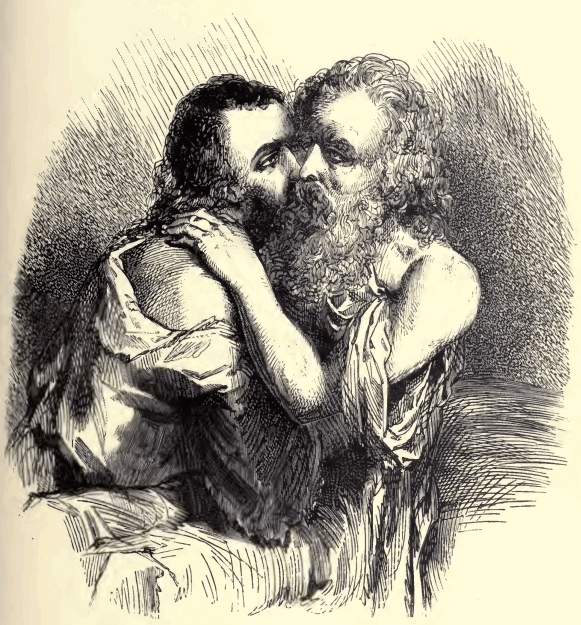
\includegraphics[width=\textwidth]{0255m.jpg}
\end{figure}

The draught produced a galvanic effect, a violent trembling pervaded
the old man’s limbs, his eyes opened until it was fearful to gaze upon
them, he heaved a sigh which resembled a shriek, and then his convulsed
body returned gradually to its former immobility, the eyes remaining
open.

Half an hour, an hour, an hour and a half elapsed, and during this
period of anguish, Edmond leaned over his friend, his hand applied to
his heart, and felt the body gradually grow cold, and the heart’s
pulsation become more and more deep and dull, until at length it
stopped; the last movement of the heart ceased, the face became livid,
the eyes remained open, but the eyeballs were glazed.

It was six o’clock in the morning, the dawn was just breaking, and its
feeble ray came into the dungeon, and paled the ineffectual light of
the lamp. Strange shadows passed over the countenance of the dead man,
and at times gave it the appearance of life. While the struggle between
day and night lasted, Dantès still doubted; but as soon as the daylight
gained the pre-eminence, he saw that he was alone with a corpse. Then
an invincible and extreme terror seized upon him, and he dared not
again press the hand that hung out of bed, he dared no longer to gaze
on those fixed and vacant eyes, which he tried many times to close, but
in vain—they opened again as soon as shut. He extinguished the lamp,
carefully concealed it, and then went away, closing as well as he could
the entrance to the secret passage by the large stone as he descended.

It was time, for the jailer was coming. On this occasion he began his
rounds at Dantès’ cell, and on leaving him he went on to Faria’s
dungeon, taking thither breakfast and some linen. Nothing betokened
that the man knew anything of what had occurred. He went on his way.

Dantès was then seized with an indescribable desire to know what was
going on in the dungeon of his unfortunate friend. He therefore
returned by the subterraneous gallery, and arrived in time to hear the
exclamations of the turnkey, who called out for help. Other turnkeys
came, and then was heard the regular tramp of soldiers. Last of all
came the governor.

Edmond heard the creaking of the bed as they moved the corpse, heard
the voice of the governor, who asked them to throw water on the dead
man’s face; and seeing that, in spite of this application, the prisoner
did not recover, they sent for the doctor. The governor then went out,
and words of pity fell on Dantès’ listening ears, mingled with brutal
laughter.

“Well, well,” said one, “the madman has gone to look after his
treasure. Good journey to him!”

“With all his millions, he will not have enough to pay for his shroud!”
said another.

“Oh,” added a third voice, “the shrouds of the Château d’If are not
dear!”

\begin{figure}[ht]
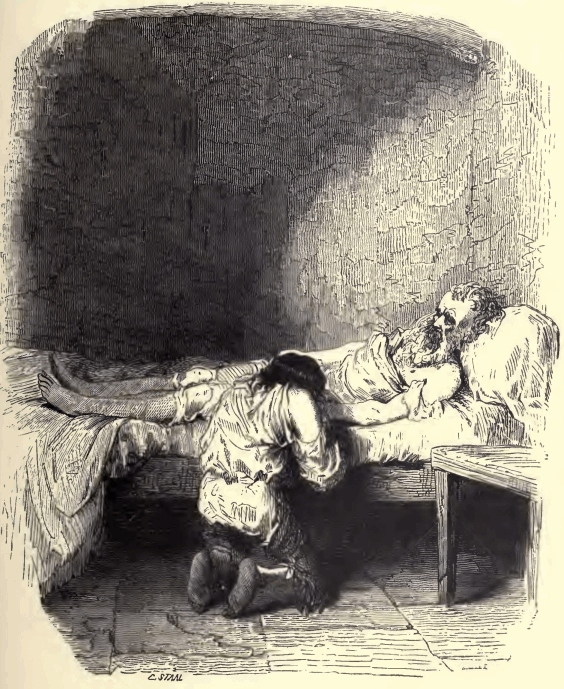
\includegraphics[width=\textwidth]{0257m.jpg}
\end{figure}

“Perhaps,” said one of the previous speakers, “as he was a churchman,
they may go to some expense in his behalf.”

“They may give him the honors of the sack.”

Edmond did not lose a word, but comprehended very little of what was
said. The voices soon ceased, and it seemed to him as if everyone had
left the cell. Still he dared not to enter, as they might have left
some turnkey to watch the dead. He remained, therefore, mute and
motionless, hardly venturing to breathe. At the end of an hour, he
heard a faint noise, which increased. It was the governor who returned,
followed by the doctor and other attendants. There was a moment’s
silence,—it was evident that the doctor was examining the dead body.
The inquiries soon commenced.

The doctor analyzed the symptoms of the malady to which the prisoner
had succumbed, and declared that he was dead. Questions and answers
followed in a nonchalant manner that made Dantès indignant, for he felt
that all the world should have for the poor abbé a love and respect
equal to his own.

“I am very sorry for what you tell me,” said the governor, replying to
the assurance of the doctor, “that the old man is really dead; for he
was a quiet, inoffensive prisoner, happy in his folly, and required no
watching.”

“Ah,” added the turnkey, “there was no occasion for watching him; he
would have stayed here fifty years, I’ll answer for it, without any
attempt to escape.”

“Still,” said the governor, “I believe it will be requisite,
notwithstanding your certainty, and not that I doubt your science, but
in discharge of my official duty, that we should be perfectly assured
that the prisoner is dead.”

There was a moment of complete silence, during which Dantès, still
listening, knew that the doctor was examining the corpse a second time.

“You may make your mind easy,” said the doctor; “he is dead. I will
answer for that.”

“You know, sir,” said the governor, persisting, “that we are not
content in such cases as this with such a simple examination. In spite
of all appearances, be so kind, therefore, as to finish your duty by
fulfilling the formalities described by law.”

“Let the irons be heated,” said the doctor; “but really it is a useless
precaution.”

This order to heat the irons made Dantès shudder. He heard hasty steps,
the creaking of a door, people going and coming, and some minutes
afterwards a turnkey entered, saying:

“Here is the brazier, lighted.”

There was a moment’s silence, and then was heard the crackling of
burning flesh, of which the peculiar and nauseous smell penetrated even
behind the wall where Dantès was listening in horror. The perspiration
poured forth upon the young man’s brow, and he felt as if he should
faint.

“You see, sir, he is really dead,” said the doctor; “this burn in the
heel is decisive. The poor fool is cured of his folly, and delivered
from his captivity.”

“Wasn’t his name Faria?” inquired one of the officers who accompanied
the governor.

\begin{figure}[ht]
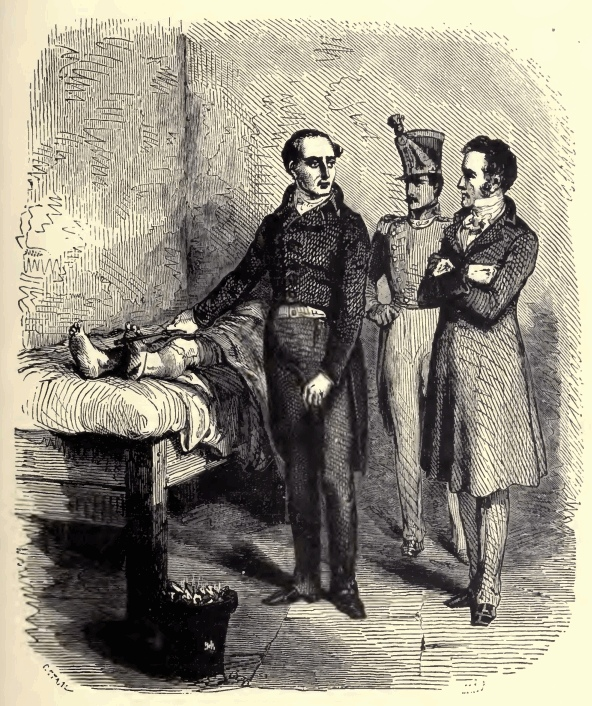
\includegraphics[width=\textwidth]{0259m.jpg}
\end{figure}

“Yes, sir; and, as he said, it was an ancient name. He was, too, very
learned, and rational enough on all points which did not relate to his
treasure; but on that, indeed, he was intractable.”

“It is the sort of malady which we call monomania,” said the doctor.

“You had never anything to complain of?” said the governor to the
jailer who had charge of the abbé.

“Never, sir,” replied the jailer, “never; on the contrary, he sometimes
amused me very much by telling me stories. One day, too, when my wife
was ill, he gave me a prescription which cured her.”

“Ah, ah!” said the doctor, “I did not know that I had a rival; but I
hope, governor, that you will show him all proper respect in
consequence.”

“Yes, yes, make your mind easy, he shall be decently interred in the
newest sack we can find. Will that satisfy you?”

“Must this last formality take place in your presence, sir?” inquired a
turnkey.

“Certainly. But make haste—I cannot stay here all day.” Other
footsteps, going and coming, were now heard, and a moment afterwards
the noise of rustling canvas reached Dantès’ ears, the bed creaked, and
the heavy footfall of a man who lifts a weight sounded on the floor;
then the bed again creaked under the weight deposited upon it.

“This evening,” said the governor.

“Will there be any mass?” asked one of the attendants.

“That is impossible,” replied the governor. “The chaplain of the
château came to me yesterday to beg for leave of absence, in order to
take a trip to Hyères for a week. I told him I would attend to the
prisoners in his absence. If the poor abbé had not been in such a
hurry, he might have had his requiem.”

“Pooh, pooh;” said the doctor, with the impiety usual in persons of his
profession; “he is a churchman. God will respect his profession, and
not give the devil the wicked delight of sending him a priest.” A shout
of laughter followed this brutal jest. Meanwhile the operation of
putting the body in the sack was going on.

“This evening,” said the governor, when the task was ended.

“At what hour?” inquired a turnkey.

“Why, about ten or eleven o’clock.”

“Shall we watch by the corpse?”

“Of what use would it be? Shut the dungeon as if he were alive—that is
all.”

Then the steps retreated, and the voices died away in the distance; the
noise of the door, with its creaking hinges and bolts ceased, and a
silence more sombre than that of solitude ensued,—the silence of death,
which was all-pervasive, and struck its icy chill to the very soul of
Dantès.

Then he raised the flag-stone cautiously with his head, and looked
carefully around the chamber. It was empty, and Dantès emerged from the
tunnel.
